\section{Konzepte und Methoden}
\label{methoden}

\subsection{Theoretische Konzepte}
\label{methoden:konzepte}

Um von den Spracherweiterungen und ihren unterschiedlichen Konzepten in Bezug
auf die Ausführung von Kerneln und die Speicherhierarchie abstrahieren zu
können, wird in diesem Abschnitt ein theoretisches GPU-Modell vorgestellt.
Dieses umfasst alle für das Verständnis der Benchmarks notwendigen Eigenschaften
einer GPU und lässt sich einfach auf die konkreten Konzepte der
Spracherweiterungen abbilden.

\subsubsection{Arbeitsgruppen und -einheiten}

Bei der Ausführung von Kerneln sind zwei Ebenen zu unterscheiden:

\begin{itemize}
    \item Eine \textbf{Arbeitseinheit} ist eine logische Instanz, die auf einen
          Hardware-Thread eines Multiprozessors abgebildet werden kann.
    \item \textbf{Arbeitsgruppen} umfassen eine unbestimmte Zahl von
          Arbeitseinheiten und werden auf die Multiprozessoren der GPU verteilt.
          Arbeitseinheiten innerhalb einer Gruppe sind untereinander
          möglicherweise asynchron, können aber durch Barrieren synchronisiert
          werden. Durch die Verteilung der Arbeitsgruppen auf die
          Multiprozessoren sind auch die Arbeitsgruppen untereinander asynchron
          und können nicht synchronisiert werden.
\end{itemize}

Die Tabelle~\ref{methoden:konzepte:arbeit:tabelle} zeigt die Abbildung der
hier vorgestellten Konzepte auf die äquivalenten Konzepte der verschiedenen
Plattformen.

\begin{table}[htb]
    \centering
    \begin{tabular}{|c|c|c|c|}
        \hline
        Modell & CUDA / HIP & HC & SYCL\\ \hline
        Arbeitsgruppe & block & tile & work group\\ \hline
        Arbeitseinheit & thread & thread & work item\\ \hline
    \end{tabular}
    \caption{Abbildung der Ausführungskonzepte des Modells auf die
             Entsprechungen der Spracherweiterungen}
    \label{methoden:konzepte:arbeit:tabelle}
\end{table}

\subsubsection{Speicherhierarchie}
\label{methoden:konzepte:speicher}

Das theoretische GPU-Modell kennt drei Ebenen der Speicherhierarchie:

\begin{itemize}
    \item Die höchste Ebene ist der \textbf{globale Speicher}. Er entspricht dem
          globalen (GDDR- oder HBM-) Speicher auf realen GPUs, ist im Modell
          jedoch unendlich groß, während die Zugriffszeit sehr langsam ist.
    \item Die nächste Ebene ist der \textbf{lokale Speicher}. Dieser hat in der
          realen Welt unterschiedlich benannte Entsprechungen
          (siehe Tabelle~\ref{methoden:konzepte:speicher:tabelle}), meint aber
          immer den schnellen Speicher, der einer Arbeitsgruppe zugeordnet ist.
          Er ist in der Kapazität beschränkt und deutlich kleiner als der
          globale Speicher, während er wesentlich schnellere Zugriffe
          ermöglicht.
    \item Auf der untersten Ebene befinden sich die \textbf{Register}, die jeder
          Ausführungseinheit in unbegrenzter Zahl zugeordnet sind. Wie in der
          realen Welt sind sie nicht direkt vom Programmierer ansprechbar. Der
          Modell-Compiler platziert in ihnen lokale Variablen der
          Arbeitseinheiten.
\end{itemize}

\begin{table}[htb]
    \centering
    \begin{tabular}{|c|c|c|c|}
        \hline
        Modell & CUDA / HIP & HC & SYCL\\ \hline
        globaler Speicher & global memory & global memory & global memory\\
        \hline
        lokaler Speicher & shared memory & \texttt{tile\_static} memory &
        local memory \\
        \hline
        Register & register & register & -\\ \hline
    \end{tabular}
    \caption{Abbildung des Speicherkonzepte des Modells auf die Entsprechungen
             der Spracherweiterungen}
    \label{methoden:konzepte:speicher:tabelle}
\end{table}

\subsubsection{Kernelsprache}

Die in den vorherigen Abschnitten entwickelten Konzepte werden für die
theoretische Beschreibung der verwendeten Benchmarks in eine fiktive
Kernel-Sprache integriert. Bei dieser Sprache handelt es sich um normales C++
mit folgenden Erweiterungen:

\begin{itemize}
    \item Das Schlüsselwort \texttt{local} markiert Variablen und Arrays, die im
          lokalen Speicher liegen.
    \item Der Befehl \texttt{synchronize()} wirkt als Barriere innerhalb einer
          Arbeitsgruppe. Es wird garantiert, dass alle vorherigen Zugriffe auf
          den (globalen und lokalen) Speicher und Rechenoperationen
          abgeschlossen wurden, bevor die Arbeitseinheiten die Befehle nach der
          Barriere ausführen können.
    \item Das Schlüsselwort \texttt{num\_groups} ist eine Variable, die die
          Anzahl aller Arbeitsgruppen enthält.
    \item Das Schlüsselwort \texttt{group\_idx} dient der eindeutigen
          Identifikation einer Arbeitsgruppe in Form einer ganzen Zahl. Die
          Indices sind fortlaufend, d.h.\ die erste Arbeitsgruppe hat den
          Index 0, die zweite den Index 1 und die $n$-te Arbeitsgruppe den
          Index $n - 1$.
    \item Das Schlüsselwort \texttt{group\_dim} ist eine Variable, die die
          Anzahl der Arbeitseinheiten einer Gruppe beinhaltet.
    \item Das Schlüsselwort \texttt{unit\_idx} dient der eindeutigen
          Identifikation einer Arbeitseinheit innerhalb einer Arbeitsgruppe. Die
          erste Einheit einer Gruppe trägt den Index 0, die zweite den Index 1
          und die $n$-te Einheit den Index $n - 1$.
    \item Die globale Position einer Arbeitseinheit, also die eindeutige
          Identifikation über Gruppengrenzen hinweg, lässt sich mit Hilfe der
          vorgegebenen Schlüsselworte berechnen:\\
          \texttt{global\_id = group\_idx * group\_dim + unit\_idx}
    \item Vektoren werden in der Form \texttt{typZAHL} notiert, z.B.\
          \texttt{int2} oder \texttt{float4}. Der Zugriff auf die Komponenten
          erfolgt über den Punktoperator und die Angabe des Felds.
          Beispielsweise sind die Komponenten des Vektors \texttt{a} vom Typ
          \texttt{float3} durch \texttt{a.x}, \texttt{a.y} und \texttt{a.z}
          ansprechbar.
\end{itemize}

Alle Indices sind im vorgestellten Modell eindimensional, was für die hier
vorgestellten Benchmarks ausreicht.

\subsection{zcopy-Benchmark}
\label{methoden:zcopy}

Der zcopy-Benchmark geht auf einen Beitrag des Nutzers \textit{njuffa}\footnote{
Vermutlich der NVIDIA-Angestellte Norbert Juffa.} im NVIDIA-Forum zurück. Er
hat das Ziel, die tatsächlich erreichbare Speicherbandbreite des globalen
GPU-Speichers zu ermitteln, indem ein Kernel ausschließlich kombinierte Lese-
und Schreibzugriffe (16 Byte pro Thread) durchführt. (vgl.~\cite{njuffa2017})

Der Benchmark wurde für diese Arbeit übernommen und angepasst:

\begin{itemize}
    \item Es wird sowohl die kombinierte Lese- und Schreibgeschwindigkeit als
          auch die reine Schreibgeschwindigkeit gemessen, da die Kombination
          eventuell zusätzlichen Overhead im Speicher-Controller der GPU
          erzeugen kann.
    \item Während der originale Benchmark nur auf 16 Byte pro Thread zugreift,
          wurden im Rahmen dieser Arbeit auch die Bandbreiten für die
          Speichergrößen 4 Byte, 8 Byte und 32 Byte ermittelt.
\end{itemize}

Quelltext~\ref{methoden:zcopy:source} zeigt den Pseudo-Code des eingesetzten
Kernels am Beispiel von 16 Byte pro Thread.

\begin{code}
    \begin{minted}[breaklines,breakafter=\,,escapeinside=||,fontsize=\small]{c++}
void read_write(double2* a, double2* b, size_t num_elems)
{
    int stride = |\textbf{\textcolor{keyword-green}{num\_groups}}| * |\textbf{\textcolor{keyword-green}{group\_dim}}|;
    int global_id = |\textbf{\textcolor{keyword-green}{group\_dim}}| * |\textbf{\textcolor{keyword-green}{group\_idx}}| + |\textbf{\textcolor{keyword-green}{unit\_idx}}|;

    for(int i = global_id; i < num_elems; i += stride)
        b[i] = a[i];
}

void write(double2* b, size_t num_elems)
{
    int stride = |\textbf{\textcolor{keyword-green}{num\_groups}}| * |\textbf{\textcolor{keyword-green}{group\_dim}}|;
    int global_id = |\textbf{\textcolor{keyword-green}{group\_dim}}| * |\textbf{\textcolor{keyword-green}{group\_idx}}| + |\textbf{\textcolor{keyword-green}{unit\_idx}}|;

    for(int i = global_id; i < num_elems; i += stride)
        b[i] = double2{0.0, 0.0};
}
    \end{minted}
    \caption{zcopy-Benchmark}
    \label{methoden:zcopy:source}
\end{code}

\subsection{Reduction-Benchmark}
\label{methoden:reduction}

\subsubsection{Theoretischer Hintergrund}

Die Reduktion eines Arrays ist eines der klassischen Konzepte der parallelen
Programmierung. Mathematisch verbirgt sich dahinter das Reduzieren einer Menge
von Zahlen auf eine kleinere Menge von Zahlen durch eine Funktion. Als Beispiel
sei eine Menge von Zahlen $A = \{a_1, a_2, \dots, a_n\}$ gegeben. Durch die
Summenfunktion lässt sich das Ergebnis $b = \sum\limits_{i = 1}^n a_i$
ermitteln -- in Mengen ausgedrückt wurde $A$ auf $B = \{b\}$ reduziert. Auf
die gleiche Weise ließe sich die Menge $C = \{c\}$ durch eine
Multiplikationsreduktion $c = \prod\limits_{i = 1}^n a_i$ berechnen.

Ein serieller Reduktionsalgorithmus ließe sich in Form einer Schleife schreiben,
die über die Menge der Zahlen iteriert und das Ergebnis der Funktion $\oplus$
für alle aufeinander folgenden Zahlen berechnet:

\begin{algorithmic}[1]
\State $result \gets 0$
\For {$i \gets 1, n$}
    \State $result \gets result \oplus a_i$
\EndFor
\end{algorithmic}

Da die Reihenfolge der Anwendung der Funktion $\oplus$ in diesem Beispiel nicht
relevant ist, lässt sich der Algorithmus einfach parallelisieren, indem eine
Menge von $p$ Arbeitseinheiten $\oplus$ zunächst auf $p$ Paare $(a_i, a_j)$
anwendet, wobei $a_i$ und $a_j$ jeweils genau einmal zugeordnet werden ($a_i$
wird also niemals zweimal verwendet). Im nächsten Schritt führen
$\frac{p}{2}$ Einheiten die Funktion erneut auf den Ergebnissen des vorherigen
Schritts aus, usw. Die Abbildung~\ref{methoden:reduction:viz} visualisiert
den Vorgang für acht Elemente $a_1, \dots, a_8$ auf das Ergebnis $b$ durch vier
Ausführungseinheiten $E_1, \dots, E_4$.

\begin{figure}[htb]
    \centering
    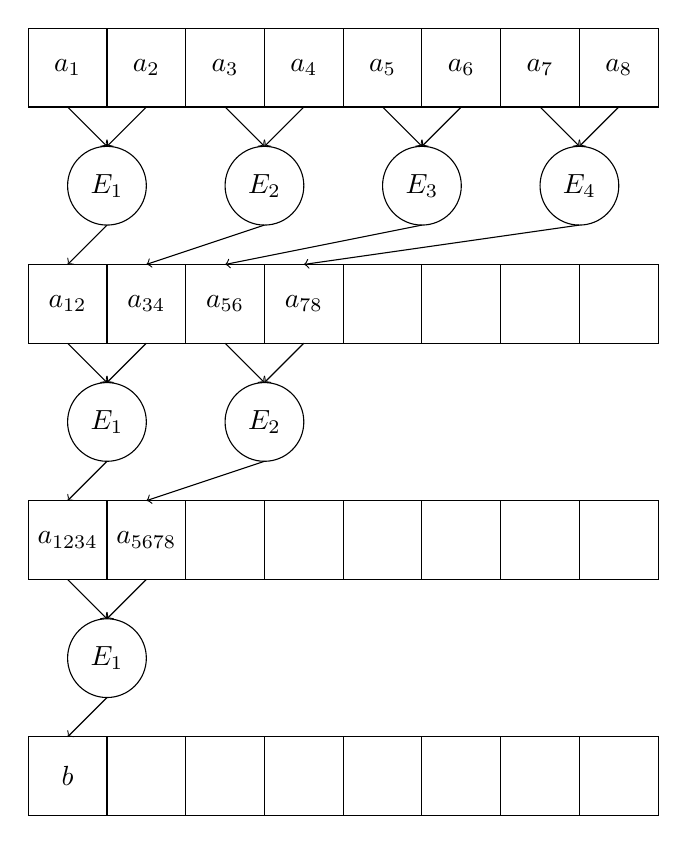
\begin{tikzpicture}
        \draw (0.0, 0.0) rectangle (1.0, -1.0) node [pos = 0.5] {$a_1$};
        \draw (1.0, 0.0) rectangle (2.0, -1.0) node [pos = 0.5] {$a_2$};
        \draw (2.0, 0.0) rectangle (3.0, -1.0) node [pos = 0.5] {$a_3$};
        \draw (3.0, 0.0) rectangle (4.0, -1.0) node [pos = 0.5] {$a_4$};
        \draw (4.0, 0.0) rectangle (5.0, -1.0) node [pos = 0.5] {$a_5$};
        \draw (5.0, 0.0) rectangle (6.0, -1.0) node [pos = 0.5] {$a_6$};
        \draw (6.0, 0.0) rectangle (7.0, -1.0) node [pos = 0.5] {$a_7$};
        \draw (7.0, 0.0) rectangle (8.0, -1.0) node [pos = 0.5] {$a_8$};

        \draw (1.0, -2.0) circle [radius = 0.50] node {$E_1$};
        \draw (3.0, -2.0) circle [radius = 0.50] node {$E_2$};
        \draw (5.0, -2.0) circle [radius = 0.50] node {$E_3$};
        \draw (7.0, -2.0) circle [radius = 0.50] node {$E_4$};

        \draw [->] (0.5, -1.0) -- (1.0, -1.5);
        \draw [->] (1.5, -1.0) -- (1.0, -1.5);
        \draw [->] (2.5, -1.0) -- (3.0, -1.5);
        \draw [->] (3.5, -1.0) -- (3.0, -1.5);
        \draw [->] (4.5, -1.0) -- (5.0, -1.5);
        \draw [->] (5.5, -1.0) -- (5.0, -1.5);
        \draw [->] (6.5, -1.0) -- (7.0, -1.5);
        \draw [->] (7.5, -1.0) -- (7.0, -1.5);

        \draw [->] (1.0, -2.5) -- (0.5, -3.0);
        \draw [->] (3.0, -2.5) -- (1.5, -3.0);
        \draw [->] (5.0, -2.5) -- (2.5, -3.0);
        \draw [->] (7.0, -2.5) -- (3.5, -3.0);

        \draw (0.0, -3.0) rectangle (1.0, -4.0) node [pos = 0.5] {$a_{12}$};
        \draw (1.0, -3.0) rectangle (2.0, -4.0) node [pos = 0.5] {$a_{34}$};
        \draw (2.0, -3.0) rectangle (3.0, -4.0) node [pos = 0.5] {$a_{56}$};
        \draw (3.0, -3.0) rectangle (4.0, -4.0) node [pos = 0.5] {$a_{78}$};
        \draw (4.0, -3.0) rectangle (5.0, -4.0);
        \draw (5.0, -3.0) rectangle (6.0, -4.0);
        \draw (6.0, -3.0) rectangle (7.0, -4.0);
        \draw (7.0, -3.0) rectangle (8.0, -4.0);

        \draw (1.0, -5.0) circle [radius = 0.50] node {$E_1$};
        \draw (3.0, -5.0) circle [radius = 0.50] node {$E_2$};

        \draw [->] (0.5, -4.0) -- (1.0, -4.5);
        \draw [->] (1.5, -4.0) -- (1.0, -4.5);
        \draw [->] (2.5, -4.0) -- (3.0, -4.5);
        \draw [->] (3.5, -4.0) -- (3.0, -4.5);

        \draw [->] (1.0, -5.5) -- (0.5, -6.0);
        \draw [->] (3.0, -5.5) -- (1.5, -6.0);

        \draw (0.0, -6.0) rectangle (1.0, -7.0) node [pos = 0.5] {$a_{1234}$};
        \draw (1.0, -6.0) rectangle (2.0, -7.0) node [pos = 0.5] {$a_{5678}$};
        \draw (2.0, -6.0) rectangle (3.0, -7.0);
        \draw (3.0, -6.0) rectangle (4.0, -7.0);
        \draw (4.0, -6.0) rectangle (5.0, -7.0);
        \draw (5.0, -6.0) rectangle (6.0, -7.0);
        \draw (6.0, -6.0) rectangle (7.0, -7.0);
        \draw (7.0, -6.0) rectangle (8.0, -7.0);

        \draw (1.0, -8.0) circle [radius = 0.50] node {$E_1$};

        \draw [->] (0.5, -7.0) -- (1.0, -7.5);
        \draw [->] (1.5, -7.0) -- (1.0, -7.5);

        \draw [->] (1.0, -8.5) -- (0.5, -9.0);

        \draw (0.0, -9.0) rectangle (1.0, -10.0) node [pos = 0.5] {$b$};
        \draw (1.0, -9.0) rectangle (2.0, -10.0);
        \draw (2.0, -9.0) rectangle (3.0, -10.0);
        \draw (3.0, -9.0) rectangle (4.0, -10.0);
        \draw (4.0, -9.0) rectangle (5.0, -10.0);
        \draw (5.0, -9.0) rectangle (6.0, -10.0);
        \draw (6.0, -9.0) rectangle (7.0, -10.0);
        \draw (7.0, -9.0) rectangle (8.0, -10.0);
    \end{tikzpicture}
    \caption{Visualisierung einer parallelen Reduktion}
    \label{methoden:reduction:viz}
\end{figure}

\subsubsection{GPU-Implementierung}

Im \gls{gpgpu}-Kontext ist die Reduktion früh untersucht worden. So stellte
Harris 2007 eine optimierte Reduktion für CUDA vor (vgl.~\cite{harris2007}). 
Eine für NVIDIAs Kepler-Architektur optimierte Variante der Reduktion wurde 2014
von Luitjens präsentiert (vgl.~\cite{luitjens2014}). Da sich Luitjens'
Implementierung NVIDIA-spezifischer Hardware-Intrinsiken bedient, die nicht auf
jeder im Rahmen dieser Arbeit untersuchten Plattform verfügbar sind, wird hier
ein anderer Ansatz verwendet.

Der Kernel, der die Reduktion durchführt, besteht aus zwei Stufen. Während der
ersten Stufe iterieren $x$ Arbeitsgruppen mit jeweils $p$ Arbeitseinheiten über
den globalen Speicher mit $n$ Elementen. Die Arbeitseinheiten führen die
Reduktion für jedes Elementepaar aus, wobei jeder Iterationsschritt $x \cdot p$
Elemente vom vorherigen Schritt entfernt auf den Speicher zugreift. Unter der
Annahme, dass $n$ ein Vielfaches von $p$ ist, werden $y = \frac{n}{p}$
Arbeitsgruppen gebraucht. Gilt $x \leq y$ unter der Bedingung, dass $y$ ein
Vielfaches von $x$ ist, führt jede Arbeitseinheit die Reduktionsoperation im
ersten Schritt genau $y$-mal aus. Dieses Zugriffsmuster ist als
\textit{(grid-)stride loop} bekannt und ein häufig genutztes Konzept der
\gls{gpgpu}-Programmierung (vgl.~\cite{harris2013} für eine Einführung und
Erklärung der Vorteile).

Während der zweiten Stufe werden die bisherigen Ergebnisse der einzelnen
Arbeitseinheiten in den lokalen Speicher geladen. Dann führt die Hälfte der
Arbeitseinheiten die Reduktionsoperation auf jeweils einem Elementepaar des
lokalen Speichers aus, dann ein Viertel auf der Arbeitseinheiten auf den neuen
Ergebnissen, usw. Am Ende gibt es pro Arbeitsgruppe genau ein Teilergebnis der
Reduktionsoperation (also $x$ Ergebnisse), das wieder in den globalen Speicher
geschrieben wird.

Durch einen erneuten Aufruf des Kernels mit einer Arbeitsgruppe und
$\frac{x}{2}$ Arbeitseinheiten lässt sich in einem weiteren Schritt das
Gesamtergebnis der Reduktion berechnen. Quelltext~\ref{methoden:reduction:code}
zeigt den Pseudo-Code des Kernels.

\begin{code}
    \begin{minted}[breaklines,breakafter=\,,escapeinside=||,fontsize=\small]{c++}
void block_reduce(const int* data, int* result, size_t num_elems)
{
    |\textbf{\textcolor{keyword-green}{local}}| int shared[p];

    int global_id = |\textbf{\textcolor{keyword-green}{group\_idx}}| * |\textbf{\textcolor{keyword-green}{group\_dim}}| + |\textbf{\textcolor{keyword-green}{unit\_idx}}|;
    int tsum = data[global_id]; // vermeide neutrales Element
    int grid_size = |\textbf{\textcolor{keyword-green}{group\_dim}}| * |\textbf{\textcolor{keyword-green}{num\_blocks}}|;
    global_id += grid_size;

    // 1. Stufe: grid-stride loop
    while((global_id + 3 * grid_size) < num_elems)
    {
        tsum += data[global_id] + data[global_id + grid_size] +
                data[global_id + 2 * grid_size] +
                data[global_id + 3 * grid_size];
        i += 4 * grid_size;
    }

    // verbleibende Elemente, falls n kein Vielfaches von p ist
    while(global_id < num_elems)
    {
        tsum += data[global_id];
        global_id += grid_size;
    }

    // schreibe Ergebnis in lokalen Speicher
    shared[|\textbf{\textcolor{keyword-green}{unit\_idx}}|] = tsum; 
    |\textbf{\textcolor{keyword-green}{synchronize}}|();

    // 2. Stufe: Reduktion innerhalb der Gruppe
    for(int bs = |\textbf{\textcolor{keyword-green}{group\_dim}}|, bsup = (|\textbf{\textcolor{keyword-green}{group\_dim}}| + 1) / 2;
        bs > 1;
        bs /= 2, bsup = (bs + 1) / 2)
    {
        bool cond = |\textbf{\textcolor{keyword-green}{unit\_idx}}| < bsup // erste Gruppenhälfte
            && |\textbf{\textcolor{keyword-green}{unit\_idx}}| + bsup < |\textbf{\textcolor{keyword-green}{group\_dim}}|
            && (|\textbf{\textcolor{keyword-green}{group\_idx}}| * |\textbf{\textcolor{keyword-green}{group\_dim}}| + |\textbf{\textcolor{keyword-green}{unit\_idx}}| + bsup) < num_elems;

        if(cond) shared[|\textbf{\textcolor{keyword-green}{unit\_idx}}|] += shared[|\textbf{\textcolor{keyword-green}{unit\_idx}}| + bsup];
        |\textbf{\textcolor{keyword-green}{synchronize}}|();
    }
    
    // Ergebnis in globalen Speicher schreiben
    if(|\textbf{\textcolor{keyword-green}{unit\_idx}}| == 0) result[|\textbf{\textcolor{keyword-green}{group\_idx}}|] = shared[0];
}
    \end{minted}
    \caption{Reduction-Benchmark}
    \label{methoden:reduction:code}
\end{code}

\subsection{N-Body-Benchmark}
\label{methoden:nbody}

\subsubsection{Vorbemerkung}
\label{methoden:nbody:vorbemerkung}

Eine effiziente Implementierung einer N-Body-Simulation mit quadratischer
Komplexität für GPUs wurde 2007 von Nyland et al.\ vorgestellt. Der in dieser
Arbeit verwendete Benchmark folgt dieser Implementierung, die theoretische
Beschreibung ist (gekürzt) ebenfalls der Arbeit von Nyland et al.\ entnommen.
(vgl.~\cite{nguyen2007})

\subsubsection{Einführung}
\label{methoden:nbody:einfuehrung}

N-Body-Simulationen wenden numerische Methoden an, um die Entwicklung eines
Systems vieler miteinander interagierender Körper zu approximieren.
N-Body-Probleme sind in den Naturwissenschaften zahlreich vertreten,
beispielsweise bei der Simulation vieler Galaxien oder Sterne und deren
Wechselwirkungen durch die Schwerkraft.

Eine N-Body-Simulation aller Körperpaare ist eine \textit{brute-force}-Technik,
die alle paarweisen Interaktionen auswertet. Aufgrund der quadratischen
Komplexität $\mathcal{O}(n^2)$ ist die Rechenlast bei großen Systemen sehr hoch:
ein System mit \num{16384} Körpern, das 20 Zeitschritte pro Sekunde simuliert,
berechnet über fünf Milliarden Interaktionen pro Sekunde. Aus diesem Grund ist
eine solche Simulation ein interessantes Ziel für den Einsatz paralleler
Beschleuniger.

\subsubsection{Mathematischer Hintergrund}
\label{methoden:nbody:mathematik}

In der in dieser Arbeit verwendeten Simulation wird das Gravitationspotential
aller Körper berechnet. Die in den folgenden Formeln vorkommenden Vektoren
werden in der Form $\vec{a}, \vec{b}, \vec{c}$ notiert und sind grundsätzlich
dreidimensional.

In einem System aus $N$ Körpern mit der Startposition $\vec{x}_i$ und der
Geschwindigkeit $\vec{v}_i$ ($1 \leq i \leq N$) ergibt sich die auf den Körper
$i$ durch die Anziehungskraft des Körpers $j$ wirkende Kraft $\vec{f}_{ij}$ wie
folgt:

\[
    \vec{f}_{ij} = G \frac{m_i m_j}{|\vec{r}_{ij}|^2} \cdot
                   \frac{\vec{r}_{ij}}{|\vec{r}_{ij}|},
\]

wobei $m_i$ und $m_j$ die Massen der Körper $i$ und $j$ sind,
$\vec{r}_{ij} = \vec{x}_j - \vec{x}_i$ der Vektor vom Körper $i$ zum Körper $j$
ist und $G$ die Gravitationskonstante darstellt. Der linke Faktor -- der
\textit{Betrag} der Kraft -- ist proportional zum Produkt der Massen und
schrumpft mit zunehmendem Abstand zwischen den Körpern $i$ und $j$. Der rechte
Faktor ist die \textit{Richtung} der Kraft. Aufgrund der anziehenden Wirkung
zwischen den Körpern $i$ und $j$ ist dieser Vektor ist ein Einheitsvektor.

Die gesamte auf den Körper $i$ wirkende Kraft $\vec{F}_i$, die sich aus den
Interaktionen mit den anderen $N - 1$ Körpern ergibt, ist die Summe aller
Interaktionen:

\[
    \vec{F}_i = \sum\limits_{\substack{1 \leq j \leq N\\ j \neq i}} \vec{f}_{ij}
              = G m_i \cdot \sum\limits_{\substack{1 \leq j \leq N\\j \neq i}}
                \frac{m_j \vec{r}_{ij}}{|\vec{r}_{ij}|^3}.
\]

Wenn sich Körper einander nähern, wächst die zwischen ihnen wirkende Kraft bis
ins Unendliche, was bei der numerischen Integration unerwünscht ist. In
astrophysikalischen Simulationen werden daher Kollisionen zwischen Körpern
grundsätzlich ausgeschlossen. Aus diesem Grund wird ein Schwächungsfaktor
$\varepsilon^2 > 0$ hinzugefügt und der Nenner wie folgt umgeschrieben:

\[
    \vec{F}_i \approx G m_i \cdot \sum\limits_{1 \leq j \leq N}
                      \frac{m_j \vec{r}_{ij}}
                           {\sqrt{|\vec{r}_{ij}|^2 + \varepsilon^2}^3}.
\]

Die Bedingung $j \neq i$ wird bei der Summe nicht länger benötigt, da
$\vec{f}_{ii} = 0$, wenn $\varepsilon^2 > 0$. Der Schwächungsfaktor stellt die
Interaktion zwischen zwei Plummer-Massepunkten dar, also Massen, die sich wie
kugelförmige Galaxien verhalten (vgl.~\cite{aarseth2003} und \cite{dyer1993}).
Effektiv beschränkt der Schwächungsfaktor die Größe der Kräfte zwischen Körpern,
was bei der numerischen Integration wünschenswert ist.

Um über die Zeit zu integrieren, muss die Beschleunigung
$\vec{a}_i = \frac{\vec{F}_i}{m_i}$ auf die Position und Geschwindigkeit des
Körpers $i$ angewendet werden, wodurch sich die Berechnung weiter vereinfacht:

\[
    \vec{a}_i \approx G \cdot \sum\limits_{1 \leq j \leq N}
                      \frac{m_j \vec{r}_{ij}}
                           {\sqrt{|\vec{r}_{ij}|^2 + \varepsilon^2}^3}
\]

Der numerische Integrator, der die Positionen und Geschwindigkeiten
aktualisiert und auch in dieser Arbeit zum Einsatz kommt, ist ein
Leapfrog-Verlet-Integrator (vgl.~\cite{verlet1967}). Er ist auf dieses Problem
anwendbar und berechnungseffizient, d.h. die Genauigkeit ist im Verhältnis zum
Rechenaufwand hoch. Die Wahl der Integrationsmethode für N-Body-Simulationen
hängt vom beobachteten System ab. Der Integrator wird in den Messungen mit
erfasst, in dieser Arbeit jedoch nicht gesondert beschrieben, da er eine lineare
Komplexität von $\mathcal{O}(n)$ besitzt und mit zunehmendem $n$ bedeutungslos
wird.

\subsubsection{GPU-Implementierung}
\label{methoden:nbody:gpu}

Den vorgestellten Algorithmus kann man sich als Berechnung jedes Feldes
$\vec{f}_{ij}$ in einem Gitter der Größe $N \times N$ vorstellen. In diesem Fall
ist die Gesamtkraft $\vec{F}_i$ bzw.\ die Beschleunigung $\vec{a}_i$ eines
Körpers $i$ die Summe aller Einträge der Zeile $i$. Jeder Eintrag kann
unabhängig von den anderen berechnet werden, was einen möglichen
Parallelisierungsgrad von $\mathcal{O}(n^2)$ ergibt. Dieser Ansatz hätte eine
Speicherkomplexität von ebenfalls $\mathcal{O}(n^2)$ zur Folge, was die
Performanz durch die verfügbare Speicherbandbreite limitieren würde. Stattdessen
werden einige Berechnungen serialisiert, um durch die Wiederverwendungen von
Daten die benötigte Speicherbandbreite zu verringern und die höchstmögliche
Leistung der arithmetischen Einheiten zu erreichen.

Das Gitter wird dazu in quadratische Kacheln gleicher Größe aufgeteilt, die aus
$p$ Zeilen und $p$ Spalten bestehen. $2p$ Körperbeschreibungen werden benötigt,
um alle $p^2$ Interaktionen innerhalb der Kachel zu berechnen, von denen $p$
wiederverwendet werden können. Diese Beschreibungen können dadurch im lokalen
Speicher oder in den Registern der auf der GPU verbauten Multiprozessoren
gehalten werden. Der Effekt der Interaktionen auf die $p$ Körper innerhalb der
Kachel wird als Aktualisierung von $p$ Beschleunigungsvektoren gespeichert.

Um die Daten effizient wiederverwenden zu können, erfolgen die Berechnungen
in einer Zeile in sequentieller Reihenfolge, während die einzelnen Zeilen
parallel berechnet werden. Abbildung~\ref{methoden:nbody:gpu:kacheln} zeigt
links die Ausführungsstrategie und rechts die Ein- und Ausgabewerte einer
Kachel.

\begin{figure}[htb]
    \centering
    \begin{tikzpicture}
        %
        % ERSTES QUADRAT
        %

        % Farbe
        \fill [color = olive] (0.5, -0.5) rectangle (1.0, -2.5); % erste Spalte
        \fill [color = teal] (1.0, -0.5) rectangle (2.5, -2.5); % Rest

        % Rand
        \draw [line width = 1.2pt] (0.5, -0.5) rectangle (2.5, -2.5);

        % Zeilen
        \draw (0.5, -1.0) -- (2.5, -1.0); % Erste Zeile
        \draw (0.5, -1.5) -- (2.5, -1.5); % Zweite Zeile
        \draw (0.5, -2.0) -- (2.5, -2.0); % Dritte Zeile

        % Spalten
        \draw (1.0, -0.5) -- (1.0, -2.5); % Erste Spalte
        \draw (1.5, -0.5) -- (1.5, -2.5); % Zweite Spalte
        \draw (2.0, -0.5) -- (2.0, -2.5); % Dritte Spalte

        % Beschriftung oben
        \draw [->, line width = 1.2pt]
              (0.5, 0.0) -- (2.5, 0.0)
              node[pos = 0.5, align = center, above] {sequentiell};

        % Beschriftung links
        \draw [<->, line width = 1.2pt]
              (0.0, -2.5) -- (0.0, -0.5)
              node[pos = 0.5, align = center, above, sloped] {parallel};

        % Pfeil - erste Zeile
        \draw [->, dashed, line width = 1.2pt, draw = orange]
              (0.75, -0.75) -- (2.25, -0.75);
        \fill [color = orange] (0.75, -0.75) circle [radius = 0.125];

        % Pfeil - zweite Zeile
        \draw [->, dashed, line width = 1.2pt, draw = orange]
              (0.75, -1.25) -- (2.25, -1.25);
        \fill [color = orange] (0.75, -1.25) circle [radius = 0.125];

        % Pfeil - erste Zeile
        \draw [->, dashed, line width = 1.2pt, draw = orange]
              (0.75, -1.75) -- (2.25, -1.75);
        \fill [color = orange] (0.75, -1.75) circle [radius = 0.125];

        % Pfeil - erste Zeile
        \draw [->, dashed, line width = 1.2pt, draw = orange]
              (0.75, -2.25) -- (2.25, -2.25);
        \fill [color = orange] (0.75, -2.25) circle [radius = 0.125];

        %
        % ZWEITES QUADRAT
        %

        % Farbe
        \fill [color = olive] (7.5, -0.5) rectangle (8.0, -2.5); % erste Spalte
        \fill [color = teal] (8.0, -0.5) rectangle (9.5, -2.5); % Rest

        % Rand
        \draw [line width = 1.2pt] (7.5, -0.5) rectangle (9.5, -2.5);

        % Zeilen
        \draw (7.5, -1.0) -- (9.5, -1.0); % Erste Zeile
        \draw (7.5, -1.5) -- (9.5, -1.5); % Zweite Zeile
        \draw (7.5, -2.0) -- (9.5, -2.0); % Dritte Zeile

        % Spalten
        \draw (8.0, -0.5) -- (8.0, -2.5); % Erste Spalte
        \draw (8.5, -0.5) -- (8.5, -2.5); % Zweite Spalte
        \draw (9.0, -0.5) -- (9.0, -2.5); % Dritte Spalte

        % Beschriftung oben
        \draw [->, >={Triangle[width=3mm,length=3mm]}, color = magenta,
               line width = 2mm, text = black]
              (8.5, 1.0) -- (8.5, -0.25)
              node [pos = 0.5, right, align = left]
              {$p$ Körper- \\ beschreibungen};

        % Beschriftung links
        \draw [->, >={Triangle[width=3mm,length=3mm]}, color = magenta,
               line width = 2mm, text = black]
              (6.0, -1.5) -- (7.25, -1.5)

              node [pos = -0.375, above, align = right]
              {$p$ Körper-\\beschreibungen}

              node [pos = -0.375, below] {$p$ Beschleunigungen};

        % Beschriftung rechts
        \draw [->, >={Triangle[width=3mm,length=3mm]}, color = magenta,
               line width = 2mm, text = black]
              (9.75, -1.5) -- (11.0, -1.5)

              node [pos = 1.25, below, align = left]
              {$p$ aktualisierte\\Beschleunigungen};

        % Pfeil - erste Zeile
        \draw [->, dashed, line width = 1.2pt, draw = orange]
              (7.75, -0.75) -- (9.25, -0.75);
        \fill [color = orange] (7.75, -0.75) circle [radius = 0.125];

        % Pfeil - zweite Zeile
        \draw [->, dashed, line width = 1.2pt, draw = orange]
              (7.75, -1.25) -- (9.25, -1.25);
        \fill [color = orange] (7.75, -1.25) circle [radius = 0.125];

        % Pfeil - erste Zeile
        \draw [->, dashed, line width = 1.2pt, draw = orange]
              (7.75, -1.75) -- (9.25, -1.75);
        \fill [color = orange] (7.75, -1.75) circle [radius = 0.125];

        % Pfeil - erste Zeile
        \draw [->, dashed, line width = 1.2pt, draw = orange]
              (7.75, -2.25) -- (9.25, -2.25);
        \fill [color = orange] (7.75, -2.25) circle [radius = 0.125];
    \end{tikzpicture}
    \caption{Schema einer Kachel}
    \label{methoden:nbody:gpu:kacheln}
\end{figure}

Der Pseudo-Code in Quelltext~\ref{methoden:nbody:gpu:bodybodyinteraction}
dient der Berechnung der Krafteinwirkung auf einen Körper $i$ durch die
Interaktion mit dem Körper $j$ und aktualisiert die Beschleunigung $a_i$ des
Körpers $i$. Die Beschreibungen der Körper enthalten die Koordinaten in den
Feldern \texttt{x}, \texttt{y} und \texttt{z} sowie die Körpermasse im Feld
\texttt{w}. Die Berechnung einer Interaktion benötigt 20 \glspl{flop}.

\begin{code}
    \begin{minted}[breaklines,breakafter=\,,escapeinside=||,fontsize=\small]{c++}
const float epsilon2 = epsilon * epsilon;

float3 body_body_interaction(float4 i, float4 j, float3 ai)
{
    // 3 FLOPs
    float3 r = j.xyz - i.xyz;

    // 6 FLOPs
    float dist_sqr = skalarprodukt(r, r) + epsilon2;

    // 4 FLOPs (2x Multiplikation, Wurzel, Inversion 
    float inv_dist_cube = 1.0 / sqrt(dist_sqr * dist_sqr * dist_sqr);

    // 1 FLOP
    float s = j.w * inv_dist_cube;

    // 6 FLOPs -- ai und r sind Vektoren, s ist skalar
    ai += r * s;

    return ai;
}
    \end{minted}
    \caption{Berechnung der Interaktion zwischen zwei Körpern}
    \label{methoden:nbody:gpu:bodybodyinteraction}
\end{code}

Eine Kachel wird von $p$ Threads ausgewertet, wobei jeder Thread die
Beschleunigung eines Körpers als Ergebnis seiner Interaktion mit $p$ anderen
Körpern aktualisiert. Das heißt, dass $p$ Körperbeschreibungen aus dem globalen
Speicher der GPU in den lokalen Speicher des Multiprozessors geladen werden.
Jeder Thread innerhalb des Blocks wertet $p$ aufeinanderfolgende Interaktionen
aus, was $p$ aktualisierte Beschleunigungen ergibt. Der Pseudo-Code in
Quelltext~\ref{methoden:nbody:gpu:tilecalculation} zeigt diese Berechnung. Der
Parameter \texttt{my\_position} enthält die Position des Körpers, den der
aktuelle Thread auswertet, während das im lokalen Speicher liegende Array
\texttt{sh\_position} die Beschreibungen der $p$ interagierenden Körper enthält.

\begin{code}
    \begin{minted}[breaklines,breakafter=\,,escapeinside=||,fontsize=\small]
          {c++}
float3 tile_calculation(float4 my_position, float3 accel)
{
    |\textbf{\textcolor{keyword-green}{local}}| float4 sh_position[p];
    for(int i = 0; i < p; ++i)
        accel = body_body_interaction(my_position, sh_position[i],
                                      accel);

    return accel;
}
    \end{minted}
    \caption{Berechnung der Interaktionen einer Kachel mit $p \times p$
             Elementen}
    \label{methoden:nbody:gpu:tilecalculation}
\end{code}

Im hier verwendeten Benchmark verarbeitet eine Gruppe von $p$ Arbeitseinheiten
sequentiell eine Reihe von $\frac{N}{p}$ Kacheln der Größe $p \times p$. Die
Wiederverwendung von Daten wird effektiver, je länger eine Zeile wird. Die
Zeilenlänge beeinflusst gleichzeitig die Größe der aus dem globalen in den
lokalen Speicher kopierten Daten. Die Kachelgröße selbst bestimmt somit den
Bedarf an Registern und lokalem Speicher. Vor der Verarbeitung einer Kachel lädt
jede Arbeitseinheit einen Körper in den lokalen Speicher und synchronisiert mit
den anderen Arbeitseinheiten innerhalb der Arbeitsgruppe. Somit liegen vor der
Verarbeitung jeder Kachel $p$ aufeinanderfolgende Körper im lokalen Speicher.

Die Abbildung~\ref{methoden:nbody:gpu:tilecluster} zeigt eine Arbeitsgruppe,
die nacheinander mehrere Kacheln verarbeitet. In horizontaler Richtung erstreckt
sich die Zeit, während die Parallelität in vertikaler Richtung zu sehen ist. Die
fett gezeichneten Linien rahmen die Kacheln ein und zeigen gleichzeitig die
Zeitpunkte, an denen der lokale Speicher befüllt wird und die Synchronisierung
der Arbeitseinheiten erfolgt. Alle $p$ Arbeitseinheiten einer Gruppe berechnen
innerhalb einer Kachel die Kräfte, die auf $p$ Körper wirken (eine Einheit pro
Körper); bei $\frac{N}{p}$ Kacheln pro Arbeitsgruppe berechnet damit jede
Einheit alle $N$ Interaktionen pro Körper.

\begin{figure}[htb]
    \centering
    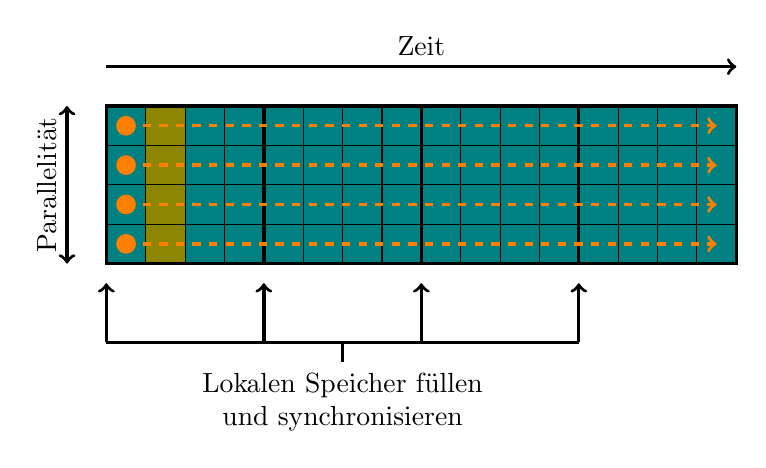
\begin{tikzpicture}
        % Farbe
        \fill [color = teal] (0.5, -0.5) rectangle (8.5, -2.5); % alles
        \fill [color = olive] (1.0, -0.5) rectangle (1.5, -2.5); % zweite Spalte

        % Rand
        \draw [line width = 1.2pt] (0.5, -0.5) rectangle (8.5, -2.5);

        % Zeilen
        \draw (0.5, -1.0) -- (8.5, -1.0); % Erste Zeile
        \draw (0.5, -1.5) -- (8.5, -1.5); % Zweite Zeile
        \draw (0.5, -2.0) -- (8.5, -2.0); % Dritte Zeile

        % Spalten
        \draw (1.0, -0.5) -- (1.0, -2.5); % Erste Spalte  (1. Q)
        \draw (1.5, -0.5) -- (1.5, -2.5); % Zweite Spalte (1. Q)
        \draw (2.0, -0.5) -- (2.0, -2.5); % Dritte Spalte (1. Q)

        \draw [line width = 1.2pt] (2.5, -0.5) -- (2.5, -2.5); % Sync #1
        
        \draw (3.0, -0.5) -- (3.0, -2.5); % Erste Spalte  (2. Q)
        \draw (3.5, -0.5) -- (3.5, -2.5); % Zweite Spalte (2. Q)
        \draw (4.0, -0.5) -- (4.0, -2.5); % Dritte Spalte (2. Q)

        \draw [line width = 1.2pt] (4.5, -0.5) -- (4.5, -2.5); % Sync #2

        \draw (5.0, -0.5) -- (5.0, -2.5); % Erste Spalte  (3. Q)
        \draw (5.5, -0.5) -- (5.5, -2.5); % Zweite Spalte (3. Q)
        \draw (6.0, -0.5) -- (6.0, -2.5); % Dritte Spalte (3. Q)

        \draw [line width = 1.2pt] (6.5, -0.5) -- (6.5, -2.5); % Sync #3

        \draw (7.0, -0.5) -- (7.0, -2.5); % Erste Spalte  (4. Q)
        \draw (7.5, -0.5) -- (7.5, -2.5); % Zweite Spalte (4. Q)
        \draw (8.0, -0.5) -- (8.0, -2.5); % Dritte Spalte (4. Q)

        % Spalten

        % Pfeil - erste Zeile
        \draw [->, dashed, line width = 1.2pt, draw = orange]
              (0.75, -0.75) -- (8.25, -0.75);
        \fill [color = orange] (0.75, -0.75) circle [radius = 0.125];

        % Pfeil - zweite Zeile
        \draw [->, dashed, line width = 1.2pt, draw = orange]
              (0.75, -1.25) -- (8.25, -1.25);
        \fill [color = orange] (0.75, -1.25) circle [radius = 0.125];

        % Pfeil - erste Zeile
        \draw [->, dashed, line width = 1.2pt, draw = orange]
              (0.75, -1.75) -- (8.25, -1.75);
        \fill [color = orange] (0.75, -1.75) circle [radius = 0.125];

        % Pfeil - erste Zeile
        \draw [->, dashed, line width = 1.2pt, draw = orange]
              (0.75, -2.25) -- (8.25, -2.25);
        \fill [color = orange] (0.75, -2.25) circle [radius = 0.125];

        % Beschriftung oben
        \draw [->, line width = 1.2pt] (0.5, 0.0) -- (8.5, 0.0)
              node [pos = 0.5, align = center, above] {Zeit};

        % Beschriftung links
        \draw [<->, line width = 1.2pt]
              (0.0, -2.5) -- (0.0, -0.5)
              node[pos = 0.5, align = center, above, sloped] {Parallelität};

        % Beschriftung unten
        \draw [line width = 1.2pt] (0.5, -3.5) -- (6.5, -3.5);
        \draw [->, line width = 1.2pt] (0.5, -3.5) -- (0.5, -2.75);
        \draw [->, line width = 1.2pt] (2.5, -3.5) -- (2.5, -2.75);
        \draw [->, line width = 1.2pt] (4.5, -3.5) -- (4.5, -2.75);
        \draw [->, line width = 1.2pt] (6.5, -3.5) -- (6.5, -2.75);
        \draw [line width = 1.2pt] (3.5, -3.5) -- (3.5, -3.75)
              node [pos = 1.0, align = center, below] {Lokalen Speicher füllen\\
              und synchronisieren};
    \end{tikzpicture}
    \caption{Berechnungen einer Arbeitsgruppe}
    \label{methoden:nbody:gpu:tilecluster}
\end{figure}

Quelltext~\ref{methoden:nbody:gpu:calcforces} zeigt den Pseudo-Code, der diese
Berechnung für GPUs umsetzt. Die Parameter \texttt{x} und \texttt{a} sind
Zeiger auf den globalen Speicher und enthalten die Positionen (\texttt{x}) und
Beschleunigungen (\texttt{a}) der Körper. Die Iteration über die Kacheln
erfordert zwei Synchronisierungspunkte. Der Erste stellt sicher, dass alle
Felder des lokalen Speichers befüllt wurden, bevor die Berechnung beginnt. Der
zweite Synchronisationspunkt garantiert, dass alle Berechnungen abgeschlossen
wurden, bevor die nächste Kachel verarbeitet wird.

\begin{code}
    \begin{minted}[breaklines,breakafter=\,,escapeinside=||,fontsize=\small]
          {c++}
void tile_calculation(float4* x, float3* a)
{
    |\textbf{\textcolor{keyword-green}{local}}| float4 sh_position[p];

    float3 acc = {0.0, 0.0, 0.0};
    int global_id = |\textbf{\textcolor{keyword-green}{group\_idx}}| * |\textbf{\textcolor{keyword-green}{group\_dim}}| + |\textbf{\textcolor{keyword-green}{unit\_idx}}|;

    float4 my_position = x[global_id];

    for(int i = 0, tile = 0; i < N; i += p, ++tile)
    {
        int idx = tile * |\textbf{\textcolor{keyword-green}{group\_dim}}| + |\textbf{\textcolor{keyword-green}{unit\_idx}}|;
        sh_position[|\textbf{\textcolor{keyword-green}{unit\_idx}}|] = x[idx];
        |\textbf{\textcolor{keyword-green}{synchronize}}|();

        acc = tile_calculation(my_position, acc);
        |\textbf{\textcolor{keyword-green}{synchronize}}|();
    }

    // Ergebnis für folgenden Integrationsschritt abspeichern
    a[global_id] = acc;
}
    \end{minted}
    \caption{Berechnung aller $N$ Interaktionen für $p$ Körper innerhalb einer
             Arbeitsgruppe mit $p$ Arbeitseinheiten}
    \label{methoden:nbody:gpu:calcforces}
\end{code}

Der gezeigte Pseudo-Code berechnet die Beschleunigung von $p$ Körpern eines
Systems, die durch ihre Interaktion mit allen $N$ Körpern im System
hervorgerufen wird. Um die Beschleunigung aller $N$ Körper zu berechnen, werden
mehrere Arbeitsgruppen eingesetzt. Da es $p$ Arbeitseinheiten pro Arbeitsgruppe
und eine Arbeitseinheit pro Körper gibt, ist die Zahl der benötigten
Arbeitsgruppen $\frac{N}{p}$. Im Gesamtsystem gibt es somit $N$
Arbeitseinheiten, die jeweils $N$ Berechnungen durchführen. Insgesamt werden
auf diese Weise $N^2$ Interaktionen berechnet. Eine Visualisierung dieses
Vorgangs findet sich in Abbildung~\ref{methoden:nbody:gpu:grid}. Die vertikale
Dimension zeigt die Parallelisierung, die durch $\frac{N}{p}$ unabhängige
Arbeitsgruppen mit jeweils $p$ Arbeitseinheiten erreicht wird. Die horizontale
Dimension zeigt die sequentielle Verarbeitung von $N$ Berechnungen durch jede
Arbeitseinheit. Eine Arbeitsgruppe lädt ihren lokalen Speicher alle $p$ Schritte
neu, um $p$ Positionen zu teilen.

\begin{figure}[htb]
    \centering
    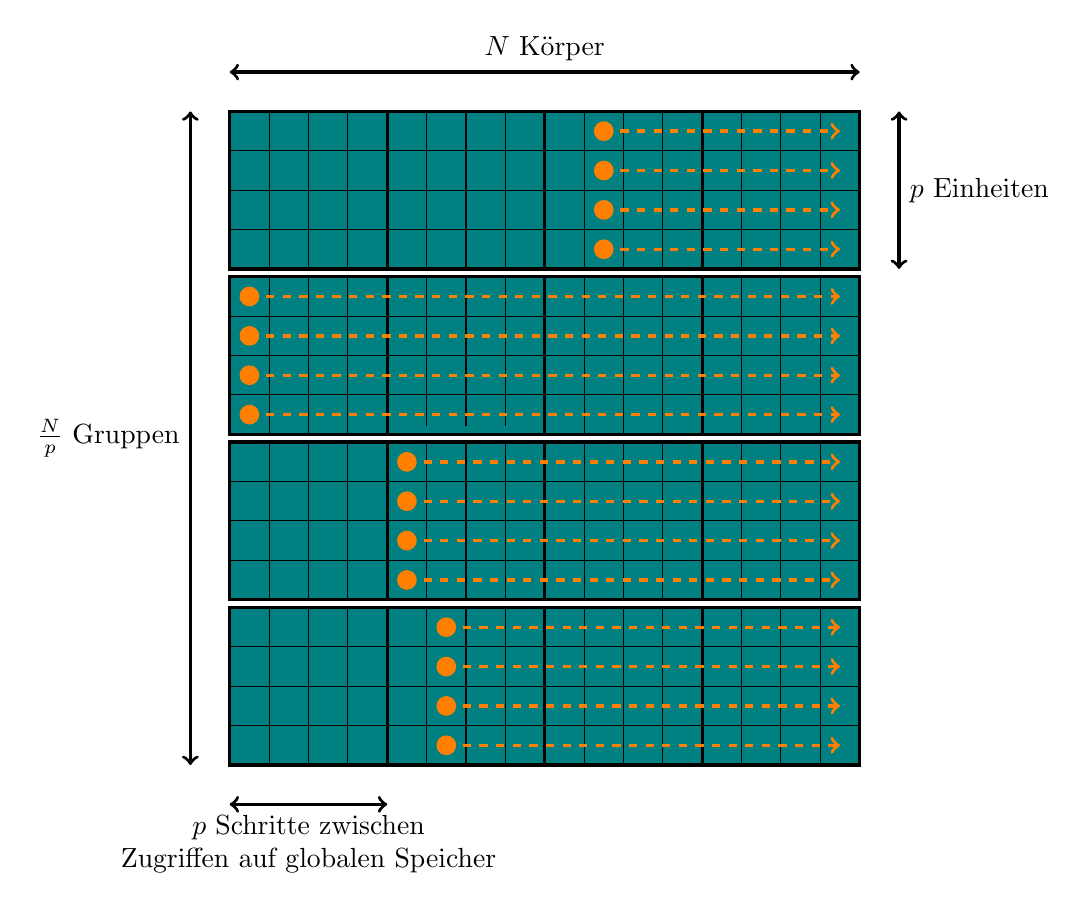
\begin{tikzpicture}
        %
        % ERSTE GRUPPE
        %

        % Farbe
        \fill [color = teal] (0.5, -0.5) rectangle (8.5, -2.5); % alles

        % Rand
        \draw [line width = 1.2pt] (0.5, -0.5) rectangle (8.5, -2.5);

        % Zeilen
        \draw (0.5, -1.0) -- (8.5, -1.0); % Erste Zeile
        \draw (0.5, -1.5) -- (8.5, -1.5); % Zweite Zeile
        \draw (0.5, -2.0) -- (8.5, -2.0); % Dritte Zeile

        % Spalten
        \draw (1.0, -0.5) -- (1.0, -2.5); % Erste Spalte  (1. Q)
        \draw (1.5, -0.5) -- (1.5, -2.5); % Zweite Spalte (1. Q)
        \draw (2.0, -0.5) -- (2.0, -2.5); % Dritte Spalte (1. Q)

        \draw [line width = 1.2pt] (2.5, -0.5) -- (2.5, -2.5); % Sync #1
        
        \draw (3.0, -0.5) -- (3.0, -2.5); % Erste Spalte  (2. Q)
        \draw (3.5, -0.5) -- (3.5, -2.5); % Zweite Spalte (2. Q)
        \draw (4.0, -0.5) -- (4.0, -2.5); % Dritte Spalte (2. Q)

        \draw [line width = 1.2pt] (4.5, -0.5) -- (4.5, -2.5); % Sync #2

        \draw (5.0, -0.5) -- (5.0, -2.5); % Erste Spalte  (3. Q)
        \draw (5.5, -0.5) -- (5.5, -2.5); % Zweite Spalte (3. Q)
        \draw (6.0, -0.5) -- (6.0, -2.5); % Dritte Spalte (3. Q)

        \draw [line width = 1.2pt] (6.5, -0.5) -- (6.5, -2.5); % Sync #3

        \draw (7.0, -0.5) -- (7.0, -2.5); % Erste Spalte  (4. Q)
        \draw (7.5, -0.5) -- (7.5, -2.5); % Zweite Spalte (4. Q)
        \draw (8.0, -0.5) -- (8.0, -2.5); % Dritte Spalte (4. Q)

        % Pfeil - erste Zeile
        \draw [->, dashed, line width = 1.2pt, draw = orange]
              (5.25, -0.75) -- (8.25, -0.75);
        \fill [color = orange] (5.25, -0.75) circle [radius = 0.125];

        % Pfeil - zweite Zeile
        \draw [->, dashed, line width = 1.2pt, draw = orange]
              (5.25, -1.25) -- (8.25, -1.25);
        \fill [color = orange] (5.25, -1.25) circle [radius = 0.125];

        % Pfeil - dritte Zeile
        \draw [->, dashed, line width = 1.2pt, draw = orange]
              (5.25, -1.75) -- (8.25, -1.75);
        \fill [color = orange] (5.25, -1.75) circle [radius = 0.125];

        % Pfeil - vierte Zeile
        \draw [->, dashed, line width = 1.2pt, draw = orange]
              (5.25, -2.25) -- (8.25, -2.25);
        \fill [color = orange] (5.25, -2.25) circle [radius = 0.125];

        %
        % ZWEITE GRUPPE
        %

        % Farbe
        \fill [color = teal] (0.5, -2.6) rectangle (8.5, -4.6);

        % Rand
        \draw [line width = 1.2pt] (0.5, -2.6) rectangle (8.5, -4.6);

        % Zeilen
        \draw (0.5, -3.1) -- (8.5, -3.1); % Erste Zeile
        \draw (0.5, -3.6) -- (8.5, -3.6); % Zweite Zeile
        \draw (0.5, -4.1) -- (8.5, -4.1); % Dritte Zeile

        % Spalten
        \draw (1.0, -2.6) -- (1.0, -4.6); % Erste Spalte  (1. Q)
        \draw (1.5, -2.6) -- (1.5, -4.6); % Zweite Spalte (1. Q)
        \draw (2.0, -2.6) -- (2.0, -4.6); % Dritte Spalte (1. Q)

        \draw [line width = 1.2pt] (2.5, -2.6) -- (2.5, -4.6); % Sync #1
        
        \draw (3.0, -2.6) -- (3.0, -4.5); % Erste Spalte  (2. Q)
        \draw (3.5, -2.6) -- (3.5, -4.5); % Zweite Spalte (2. Q)
        \draw (4.0, -2.6) -- (4.0, -4.5); % Dritte Spalte (2. Q)

        \draw [line width = 1.2pt] (4.5, -2.6) -- (4.5, -4.6); % Sync #2

        \draw (5.0, -2.6) -- (5.0, -4.6); % Erste Spalte  (3. Q)
        \draw (5.5, -2.6) -- (5.5, -4.6); % Zweite Spalte (3. Q)
        \draw (6.0, -2.6) -- (6.0, -4.6); % Dritte Spalte (3. Q)

        \draw [line width = 1.2pt] (6.5, -2.6) -- (6.5, -4.6); % Sync #3

        \draw (7.0, -2.6) -- (7.0, -4.6); % Erste Spalte  (4. Q)
        \draw (7.5, -2.6) -- (7.5, -4.6); % Zweite Spalte (4. Q)
        \draw (8.0, -2.6) -- (8.0, -4.6); % Dritte Spalte (4. Q)

        % Pfeil - erste Zeile
        \draw [->, dashed, line width = 1.2pt, draw = orange]
              (0.75, -2.85) -- (8.25, -2.85);
        \fill [color = orange] (0.75, -2.85) circle [radius = 0.125];

        % Pfeil - zweite Zeile
        \draw [->, dashed, line width = 1.2pt, draw = orange]
              (0.75, -3.35) -- (8.25, -3.35);
        \fill [color = orange] (0.75, -3.35) circle [radius = 0.125];

        % Pfeil - dritte Zeile
        \draw [->, dashed, line width = 1.2pt, draw = orange]
              (0.75, -3.85) -- (8.25, -3.85);
        \fill [color = orange] (0.75, -3.85) circle [radius = 0.125];

        % Pfeil - vierte Zeile
        \draw [->, dashed, line width = 1.2pt, draw = orange]
              (0.75, -4.35) -- (8.25, -4.35);
        \fill [color = orange] (0.75, -4.35) circle [radius = 0.125];

        %
        % DRITTE GRUPPE
        %

        % Farbe
        \fill [color = teal] (0.5, -4.7) rectangle (8.5, -6.7);

        % Rand
        \draw [line width = 1.2pt] (0.5, -4.7) rectangle (8.5, -6.7);

        % Zeilen
        \draw (0.5, -5.2) -- (8.5, -5.2); % Erste Zeile
        \draw (0.5, -5.7) -- (8.5, -5.7); % Zweite Zeile
        \draw (0.5, -6.2) -- (8.5, -6.2); % Dritte Zeile

        % Spalten
        \draw (1.0, -4.7) -- (1.0, -6.7); % Erste Spalte  (1. Q)
        \draw (1.5, -4.7) -- (1.5, -6.7); % Zweite Spalte (1. Q)
        \draw (2.0, -4.7) -- (2.0, -6.7); % Dritte Spalte (1. Q)

        \draw [line width = 1.2pt] (2.5, -4.7) -- (2.5, -6.7); % Sync #1
        
        \draw (3.0, -4.7) -- (3.0, -6.7); % Erste Spalte  (2. Q)
        \draw (3.5, -4.7) -- (3.5, -6.7); % Zweite Spalte (2. Q)
        \draw (4.0, -4.7) -- (4.0, -6.7); % Dritte Spalte (2. Q)

        \draw [line width = 1.2pt] (4.5, -4.7) -- (4.5, -6.7); % Sync #2

        \draw (5.0, -4.7) -- (5.0, -6.7); % Erste Spalte  (3. Q)
        \draw (5.5, -4.7) -- (5.5, -6.7); % Zweite Spalte (3. Q)
        \draw (6.0, -4.7) -- (6.0, -6.7); % Dritte Spalte (3. Q)

        \draw [line width = 1.2pt] (6.5, -4.7) -- (6.5, -6.7); % Sync #3

        \draw (7.0, -4.7) -- (7.0, -6.7); % Erste Spalte  (4. Q)
        \draw (7.5, -4.7) -- (7.5, -6.7); % Zweite Spalte (4. Q)
        \draw (8.0, -4.7) -- (8.0, -6.7); % Dritte Spalte (4. Q)

        % Pfeil - erste Zeile
        \draw [->, dashed, line width = 1.2pt, draw = orange]
              (2.75, -4.95) -- (8.25, -4.95);
        \fill [color = orange] (2.75, -4.95) circle [radius = 0.125];

        % Pfeil - zweite Zeile
        \draw [->, dashed, line width = 1.2pt, draw = orange]
              (2.75, -5.45) -- (8.25, -5.45);
        \fill [color = orange] (2.75, -5.45) circle [radius = 0.125];

        % Pfeil - dritte Zeile
        \draw [->, dashed, line width = 1.2pt, draw = orange]
              (2.75, -5.95) -- (8.25, -5.95);
        \fill [color = orange] (2.75, -5.95) circle [radius = 0.125];

        % Pfeil - vierte Zeile
        \draw [->, dashed, line width = 1.2pt, draw = orange]
              (2.75, -6.45) -- (8.25, -6.45);
        \fill [color = orange] (2.75, -6.45) circle [radius = 0.125];

        %
        % VIERTE GRUPPE
        %

        % Farbe
        \fill [color = teal] (0.5, -6.8) rectangle (8.5, -8.8);

        % Rand
        \draw [line width = 1.2pt] (0.5, -6.8) rectangle (8.5, -8.8);

        % Zeilen
        \draw (0.5, -7.3) -- (8.5, -7.3); % Erste Zeile
        \draw (0.5, -7.8) -- (8.5, -7.8); % Zweite Zeile
        \draw (0.5, -8.3) -- (8.5, -8.3); % Dritte Zeile

        % Spalten
        \draw (1.0, -6.8) -- (1.0, -8.8); % Erste Spalte  (1. Q)
        \draw (1.5, -6.8) -- (1.5, -8.8); % Zweite Spalte (1. Q)
        \draw (2.0, -6.8) -- (2.0, -8.8); % Dritte Spalte (1. Q)

        \draw [line width = 1.2pt] (2.5, -6.8) -- (2.5, -8.8); % Sync #1
        
        \draw (3.0, -6.8) -- (3.0, -8.8); % Erste Spalte  (2. Q)
        \draw (3.5, -6.8) -- (3.5, -8.8); % Zweite Spalte (2. Q)
        \draw (4.0, -6.8) -- (4.0, -8.8); % Dritte Spalte (2. Q)

        \draw [line width = 1.2pt] (4.5, -6.8) -- (4.5, -8.8); % Sync #2

        \draw (5.0, -6.8) -- (5.0, -8.8); % Erste Spalte  (3. Q)
        \draw (5.5, -6.8) -- (5.5, -8.8); % Zweite Spalte (3. Q)
        \draw (6.0, -6.8) -- (6.0, -8.8); % Dritte Spalte (3. Q)

        \draw [line width = 1.2pt] (6.5, -6.8) -- (6.5, -8.8); % Sync #3

        \draw (7.0, -6.8) -- (7.0, -8.8); % Erste Spalte  (4. Q)
        \draw (7.5, -6.8) -- (7.5, -8.8); % Zweite Spalte (4. Q)
        \draw (8.0, -6.8) -- (8.0, -8.8); % Dritte Spalte (4. Q)

        % Pfeil - erste Zeile
        \draw [->, dashed, line width = 1.2pt, draw = orange]
              (3.25, -7.05) -- (8.25, -7.05);
        \fill [color = orange] (3.25, -7.05) circle [radius = 0.125];

        % Pfeil - zweite Zeile
        \draw [->, dashed, line width = 1.2pt, draw = orange]
              (3.25, -7.55) -- (8.25, -7.55);
        \fill [color = orange] (3.25, -7.55) circle [radius = 0.125];

        % Pfeil - dritte Zeile
        \draw [->, dashed, line width = 1.2pt, draw = orange]
              (3.25, -8.05) -- (8.25, -8.05);
        \fill [color = orange] (3.25, -8.05) circle [radius = 0.125];

        % Pfeil - vierte Zeile
        \draw [->, dashed, line width = 1.2pt, draw = orange]
              (3.25, -8.55) -- (8.25, -8.55);
        \fill [color = orange] (3.25, -8.55) circle [radius = 0.125];

        % Beschriftung oben
        \draw [<->, line width = 1.2pt] (0.5, 0.0) -- (8.5, 0.0)
              node [pos = 0.5, align = center, above] {$N$ Körper};

        % Beschriftung links
        \draw [<->, line width = 1.2pt]
              (0.0, -8.8) -- (0.0, -0.5)
              node[pos = 0.5, left] {$\frac{N}{p}$ Gruppen};

        % Beschriftung unten
        \draw [<->, line width = 1.2pt]
              (0.5, -9.3) -- (2.5, -9.3)
              node[pos = 0.5, below, align = center]
              {$p$ Schritte zwischen\\Zugriffen auf globalen Speicher};

        % Beschriftung rechts
        \draw [<->, line width = 1.2pt]
              (9.0, -0.5) -- (9.0, -2.5)
              node[pos = 0.5, right] {$p$ Einheiten};
    \end{tikzpicture}
    \caption{Berechnung aller Interaktionen}
    \label{methoden:nbody:gpu:grid}
\end{figure}
